\documentclass[10pt]{article}
\usepackage{graphicx}
\usepackage{float}
\title{Tweak Optimization With the Mu + Lambda Evolutionary Strategy}
\date{\today}
\author{Adrian Schiller \\  Max Marti}

\begin{document}
\maketitle


\section{The Question}
 What effect would changing the amount of tweaks to each child in the Mu + Lambda Evolutionary Strategy (MPLES) have on the outcome? Unlike the Mu,Lambda Evolutionary Strategy, the MPLES keeps the parents in case they have a better fitness than the children. Keeping this in mind, having a record of the parents means that the children can be tweaked more and introduce a greater rate of change per generation.  
 
\section{The Setup}
\label{sec:setup}


Before gathering data, the algorithm was modified to allow a specifiable amount of tweaks per child between each generation. The algorithm was then run several times, each time with an incremented number of tweaks.
\begin{itemize}
\item Problem: OnesMax, with 1000 bits and 1000 iterations
\item Algorithm run with both one parent and two children, and with two and six
\item Number of tweaks ranged from one to six
\end{itemize}








\section{The Results}

\begin{table}[H]
\begin{center}
\begin{tabular}{r r}
Num Tweaks & Median Solution \\
\hline
1 & 571.5\\
2 & 598.5\\
3 & 609.5\\
4 & 618.0\\
5 & 622.0\\
6 & 626.0\\

\end{tabular}
\end{center}
\caption{Number of tweaks and their Median outcome for one Parent and six Children MPLES }
\label{tab:setup}
\end{table}





\begin{figure}[H]
•
\caption{Quality vs. Searcher for up to six tweaks, one parent, two children}
\centering
  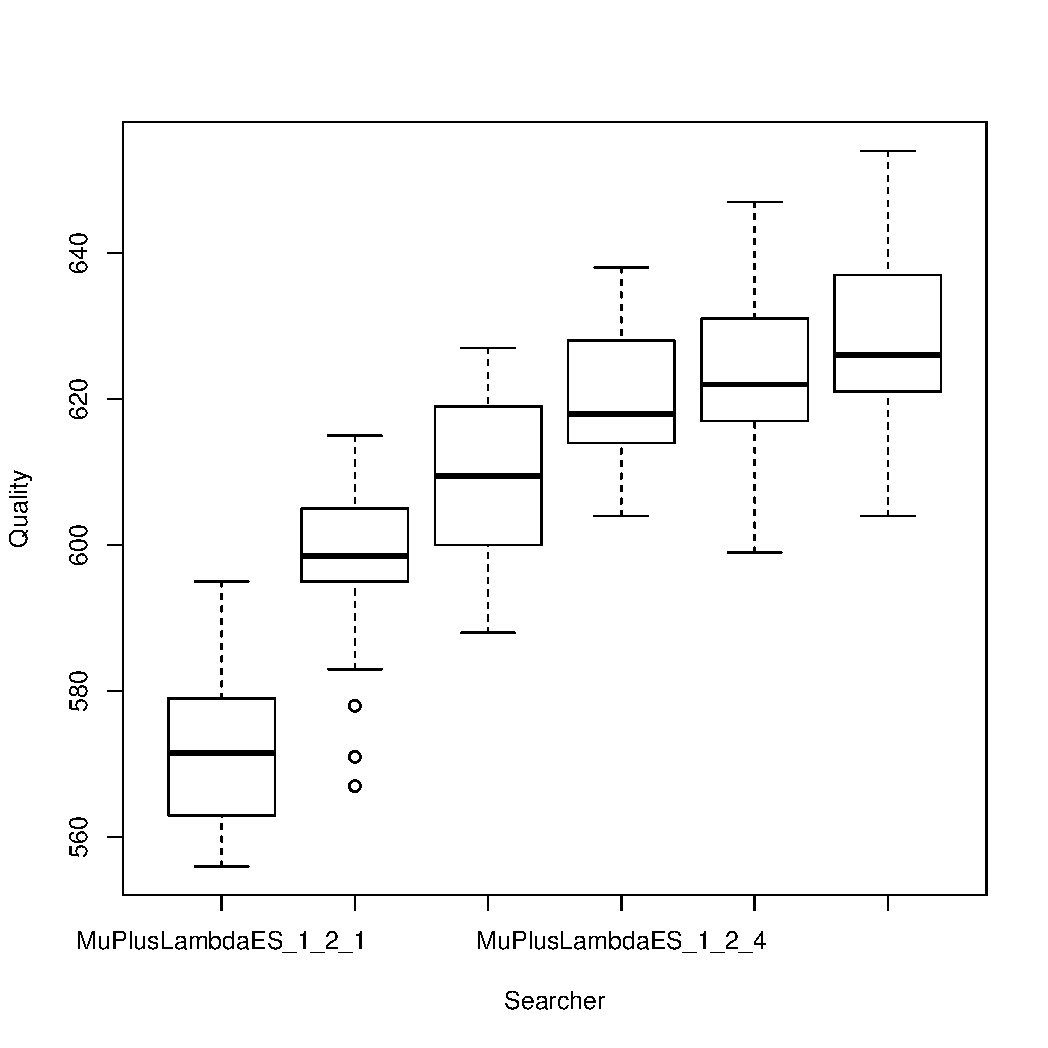
\includegraphics[scale=.65]{MuPlusLambdaTweak_1_2}
\label{fig:results}
\end{figure}

\begin{figure}[H]
•

\caption{Quality vs. Searcher for up to six tweaks, two parents, six children}
\centering
  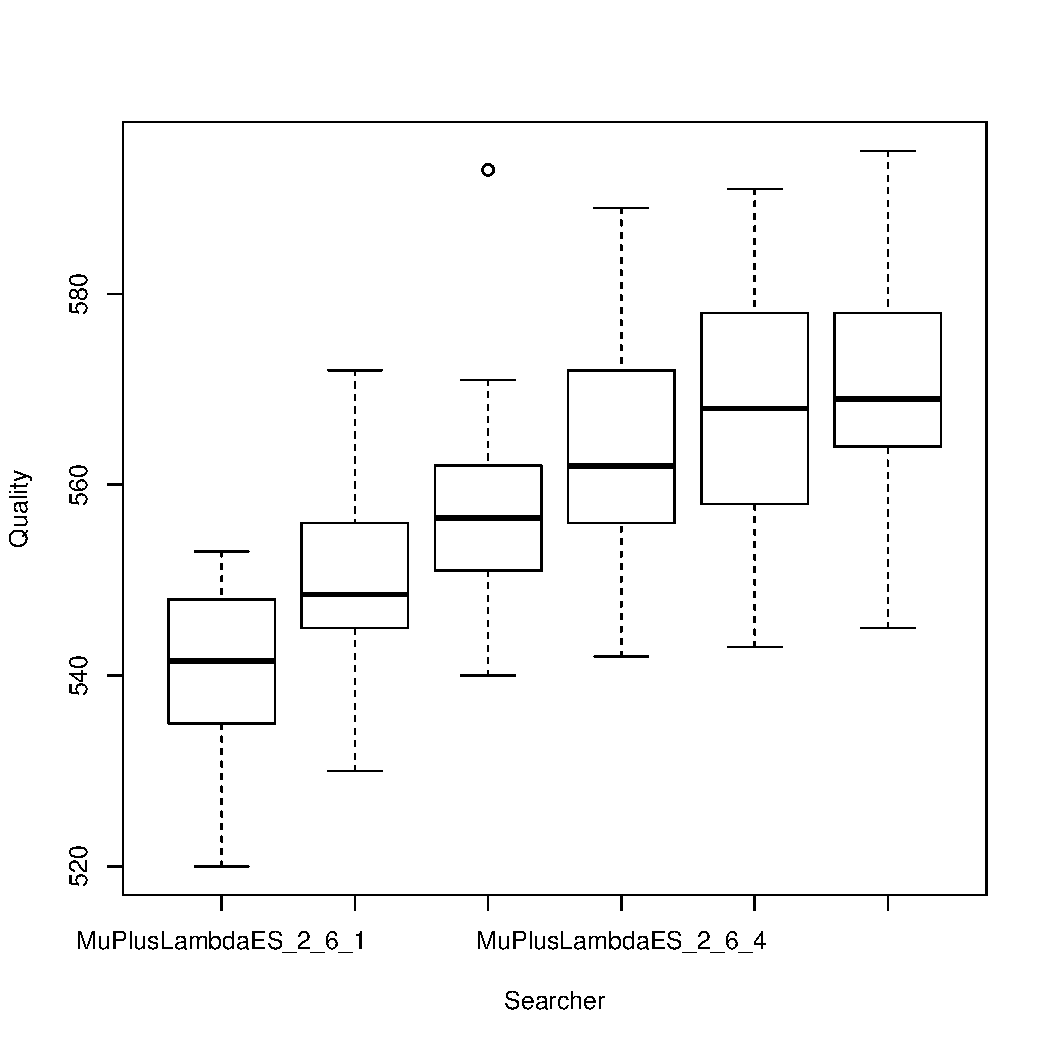
\includegraphics[scale=.65]{MuPlusLambdaTweak_2_6}
\label{fig:results}
\end{figure}

\begin{table}[H]
\begin{center}
\begin{tabular}{r r}
Num Tweaks & Median Solution \\
\hline
1 & 541.5\\
2 & 548.5\\
3 & 556.5\\
4 & 562.0\\
5 & 568.0\\
6 & 569.0\\

\end{tabular}
\end{center}
\caption{Number of tweaks and their Median outcome for two Parents and six Children MPLES }
\label{tab:setup}
\end{table}





\section{The Discussion}
The results show a positive correlation between increasing the number of tweaks and the quality of the outcome. The graphs of the data showed a log(n) curve. The rate of change decreased as the number of tweaks increased, so this method has diminishing returns. In addition, the number of tweaks, which are proportional to the number of children being generated, had a negative effect on the speed of the algorithm as they increased. It is possible that this method works because it does more operations per generation without calling additional checks to solution quality, which serves as the clock. Overall, we saw a positive, statistically significant change in the performance of the algorithm as the number of tweaks increased.
\end{document}
